\documentclass[12pt,letterpaper,twoside]{article}

\newif\ifsolution\solutiontrue   % Include the solutions
%\newif\ifsolution\solutionfalse  % Exclude the solutions

\usepackage{stats370}
\usepackage{xcolor}
\usepackage{float}
\usepackage{dsfont}
\usepackage{enumitem}
\usepackage{mathtools}
% \usepackage{breqn}
\usepackage{graphicx}
\usepackage[section]{placeins}
% \graphicspath{{output/}{\main/output/}}

\allowdisplaybreaks
\raggedbottom

\newcommand{\T}[1]{\text{\texttt{#1}}}
\newcommand{\V}[1]{\text{\textit{#1}}}

\begin{document}

{\centering \textbf{Project: Sampling Methodologies \\}}
\vspace*{-8pt}\noindent\rule{\linewidth}{1pt}

\paragraph{Purpose} of the project is to compare different sampling methodologies 
for estimating the posterior $p(\theta|y_1,...,y_n)$ of a bayesian 
inference problem.

\paragraph{Data} $(y_1,...,y_n)$ are gene expression measurements for two genes 
on $n=24$ samples where $y_i=(y_{i,1}, y_{i,2})$ represent gene expressions for 
sample i. Our samples are all labelled by "group", denoted $(t_1,...,t_n)$. 
Cell type (or mix of cell types) vary with group and we assume mean gene 
expression (but not variance) depends on cell type. Moreover, the expressions 
of different genes are independently normally distributed.

\begin{itemize}
    \item $Y_i \sim N(\mu, \sigma^2 \mathbb{I})$ if sample $i$ from group 1
    \item $Y_i \sim N(\gamma, \sigma^2 \mathbb{I})$ if sample $i$ from group 2
    \item $Y_i \sim N(0.5\mu + 0.5\gamma, \sigma^2 \mathbb{I})$ if sample $i$ from group 3
    \item $Y_i \sim N(\tau\mu + (1-\tau)\gamma, \sigma^2 \mathbb{I})$ if sample $i$ from group 4
\end{itemize}

Our model has a 6-dimensional parameter $\theta = (\sigma^2, \tau, \mu_1, \mu_2, \gamma_1, \gamma_2)$.

For all sampling methodologies, I computed 5000 samples with a 
burn-in of 200. The rest (step size, momentum, proposals, etc.) I 
discuss and treat as design choices.

\section{Metropolis Hastings}
To implement the Metropolis-Hastings algorithm we require the 
joint and transition densities to compute the hastings ratio. 
Below we derive the join density for our model, and treat the 
transition density as a design choice.

\textbf{Joint density}:
\begin{align*}
    p(\theta|y) & \propto \prod_{i=1}^n p(y|\theta) p(\theta) \\
                & = \prod_{t=1}^4 \prod_{i=1}^n 1\{t_i=t\} \cdot p(y_i|\theta) \cdot p(\mu) \cdot p(\gamma) \cdot p(\tau) \cdot p(\sigma^2) \\
                & = \prod_{t_i=1} N(\mu, \sigma^2 \mathbb{I}) \cdot \prod_{t_i=2} N(\gamma, \sigma^2 \mathbb{I}) \cdot \prod_{t_i=3} N(0.5\mu + 0.5\gamma, \sigma^2 \mathbb{I}) \cdot \prod_{t_i=4} N(\tau\mu + (1-\tau)\gamma, \sigma^2 \mathbb{I}) \cdot p(\sigma^2)
\end{align*}

\textbf{Hastings Ratio}: let $q(\theta_0, \theta_1)$ be our transition density and 
$\pi(y,\theta)$ be our join density. Then, 
$$\text{accept prob.} = \min(1, \frac{q(\theta_0, \theta_1)\pi(y,\theta_1)}{q(\theta_1, \theta_0)\pi(y,\theta_0)})$$

\begin{python}
def metropolis_hastings(data, n_samples, step_size, inital_position):
    curr_theta = inital_position.copy()
    samples = [curr_theta]

    while it < n_samples:

        proposed = proposal_sampler(curr_theta, step_size)
        h_ratio = hastings_ratio(proposed, curr_theta, data)
        accept_prob = min(1, h_ratio)

        if np.random.uniform(0, 1) <= accept_prob:
            curr_theta = proposed
            accept_count += 1

        samples.append(curr_theta)

    return samples
\end{python}

The Metropolis-Hastings algorithm itself is very simple,
However, there are still a number of design choices we need to make, 
such as (a) how to propose a new sample, (b) enforcing any constraints 
we have (e.g. $\tau \in [0,1]$), and (c) choosing hyperparameters (step 
size, burn-in).

\begin{enumerate}[label=(\alph*)]
\item \textbf{Proposal selection}: If possible, we would like to pick a symmetric 
proposal distribution to sample from (which implies a symmetric transition 
kernel) since this will simplify computation and guarantee detail balance. 
I used a gaussian random step with mean equal to the step size and variance 
of 1 which worked well (achieved reasonable acceptance ratio of 0.4-0.5).

\begin{python}
    def proposal_sampler(curr_theta, step_size):
    num_params = len(curr_theta)

    while True:
        randomness = np.random.normal(0, 1, num_params)
        proposal = curr_theta + np.multiply(step_size, randomness)

        if proposal[0] > 0 and (proposal[1] >= 0 and proposal[1] <= 1):
            break

    return proposal
\end{python}

Note: If this choice had not worked so well, I would have tried non-symmetric 
options that better mimic the expected behaviour of $tau$ and $sigma^2$ parameters
given their constraints.

\item \textbf{Enforcing constraints}: We had two constraints to consider: (a) $\sigma^2 > 0$ 
and (b) $0 \le \tau \le 1$. I enforce these constraints in the proposal sampler function 
but simply resampling if the proposal violates either (a) or (b). Note, this would be 
problematic (i.e. lead to us collecting biased posterior samples) if these constraints were 
often binding, however, we can see in the results below (figure 1) that neither $\sigma^2$ 
nor $\tau$ have maximum likelihoods or significant probability density near their boundaries 
and so the biased-ness we introduce will be minimal. 

\item \textbf{Hyperparameters}: There are not many hyperparameters to 
tune for Metropolis-Hastings, which is one of its advantages! I 
experimented with different step sizes (0.01, 0.05, 0.1, 0.5), 
and for each computed the acceptance ratio and number of 
effective (uncorrelated) samples for 300 sample test (after 
burn-in). I choose a step size of 0.05 since it maximized 
number of effective samples.

\begin{table}[h]
    \centering
    \begin{tabular}{lllll}
        Step size                   & 0.01 & 0.05  & 0.1   & 0.5   \\
        Acceptance ratio            & 0.92 & 0.45  & 0.19  & 0.02  \\
        Number of effective samples & 4.53 & 16.64 & 9.97  & 6.96  \\
                                    &      &       &       &         
    \end{tabular}
\end{table}

I did not investigate varying initialization (used $[1., 0.5, 0., 0., 0., 0.]$)
or burn-in (fixed at 200 to match what I saw in textbook examples).
\end{enumerate}

\textbf{Results}: Using the above design choices, we produce the following 
samples from our posterior (figure 1). These passed basic 
sense checks, such as $\sigma^2$ and $\tau$ falling within 
their respective bounds, lower variance as we increase number 
of samples, and minimal density on boundary of $\tau$ as hoped.
\begin{figure}[H]
    \centering
    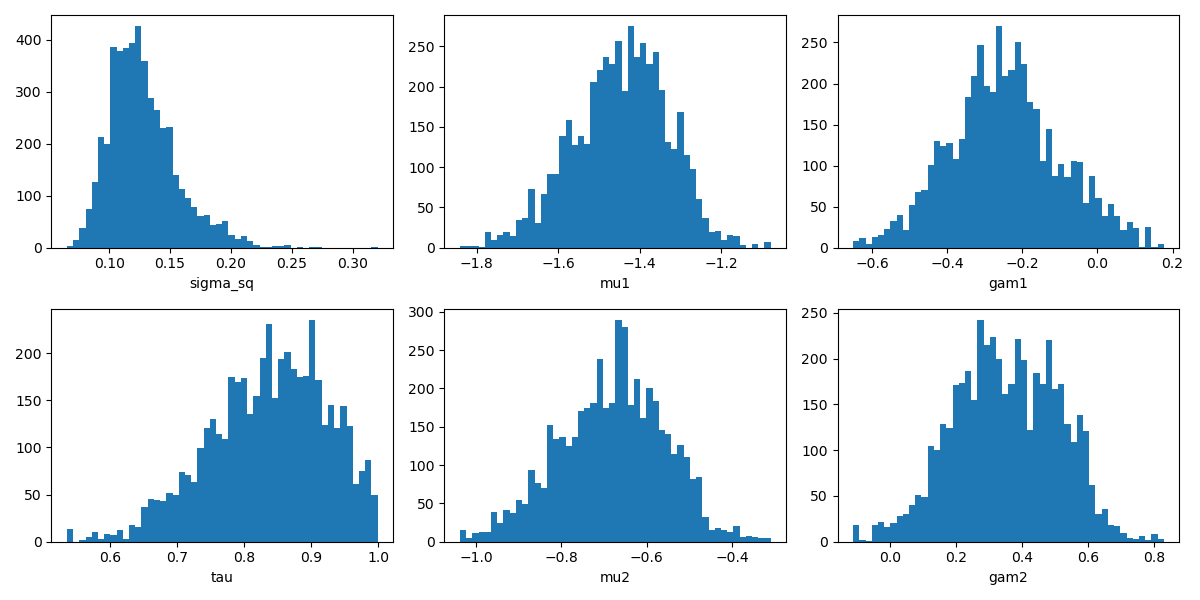
\includegraphics[scale=0.7]{mh_sampled_histogram.png}
    \caption{Histogram of Metropolis-Hastings posterior samples}
\end{figure}

The traceplots in figure 2 give an indication of how well the sampler 
explored the posterior density. I am comforted by the fact that 
there are no long periods of repeated values (getting stuck) 
despite an acceptance rate of only 0.45.
\begin{figure}[H]
    \centering
    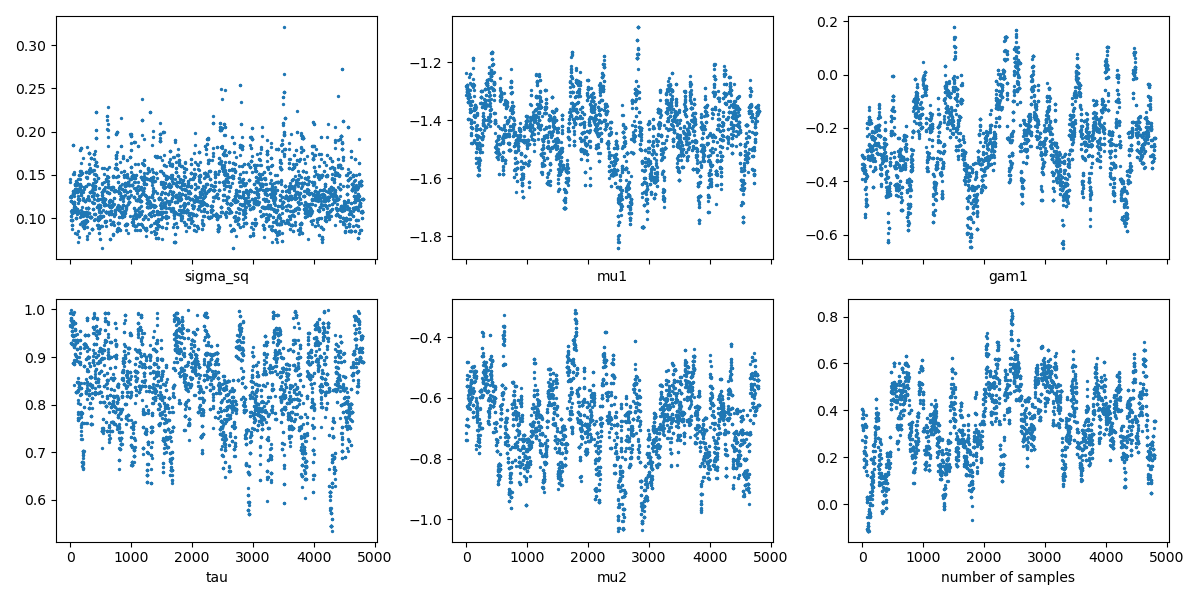
\includegraphics[scale=0.7]{mh_sampled_traceplot.png}
    \caption{Traceplot for Metropolis-Hastings sampling}
\end{figure}

\textbf{Final remarks}. Metropolis-Hastings is simple to implement 
and relatively fast to run (time = 197 sec for 5000 samples), however,
number of effective samples (autocorrelation) and acceptance ratio 
were not as good as we might expect from other technqiues that take 
more directed paths through the posterior space (e.g. HMC).   



\section{Hamiltonian Monte Carlo} 
To implement the Hamiltonian Monte Carlo we need to compute 
the Hamiltonian $H(\rho, \theta)$ given independently drawn momentum 
$\rho$ and our current paramewter values $\theta$. 
\begin{align*}
    H(\theta, y) & = -\log p(\rho, \theta) \\
                 & = - \log p(\rho|\theta) - \log p(\theta) \\
                 & = K(\rho, \theta) + V(\theta) && \text{kinetic and potential energy}
\end{align*}
We now evolve the system using the following equations from 
Hamiltonian mechanics. Note: $\frac{\partial V}{\partial \rho} = 0$ 
and if we choose our kinetic energy to be gaussian 
$K(\rho, \theta) = \frac{1}{2}\rho^T M^{-1} \rho + \log |M| + \text{const.}$ 
so we get $\frac{\partial K}{\partial \rho} = M^{-1} \rho$ and 
$\frac{\partial K}{\partial \theta} = 0$.
\begin{align*}
    \frac{d\theta}{dt} & = + \frac{\partial H}{\partial \rho} = + \frac{\partial K}{\partial \rho} + \frac{\partial V}{\partial \rho} = M^{-1} \rho \\
    \frac{d\rho}{dt}   & = - \frac{\partial H}{\partial \theta} = -\frac{\partial K}{\partial \theta} - \frac{\partial V}{\partial \theta} = -\frac{\partial V}{\partial \theta}
\end{align*}

Therefore, to implement the above system, we need only to calculate 
the gradient of our potential energy (negative log likelihood) with 
respect to our parameters $\theta$.

\textbf{Negative log likelihood}: let $V(\theta) = -l(\theta) = -\log p(\theta|y)$,
\begin{align*}
    V(\theta) & = - \log \prod_{i=1}^n p(y|\theta) p(\theta) \\
              & = - \sum_{i=1}^n \log p(y|\theta) - \log p(\theta) && \text{let $y_i'$ = centered data}\\
              & = - \sum_{i=1}^n \log \left[(2\pi)^{-k/2} \cdot |\sigma^2 \mathbb{I}|^{-1/2} \cdot \exp(\frac{-1}{2} y_i'^T (\sigma^2 \mathbb{I})^{-1} y_i')\right] - \log \frac{1}{\sigma^2} \\
              & = \frac{nk}{2} \log 2\pi + (n+1) \log \sigma^2 + \frac{1}{2\sigma^2} \sum_{i=1}^n y_i'^T \mathbb{I}^{-1} y_i'       
\end{align*}

\textbf{Gradient of $V(\theta)$ wrt $\theta$}: 
\begin{align*}
    \frac{\partial V(\theta)}{\partial \sigma^2} & = \frac{n+1}{\sigma^2} - \frac{1}{2(\sigma^2)^2}\sum_{i=1}^n \|y_i'\|^2_2 \\
    \frac{\partial V(\theta)}{\partial \tau} & = \frac{1}{\sigma^2} \cdot (\gamma - \mu)^T \sum_{t_i=4} y_i' \\
    \frac{\partial V(\theta)}{\partial \mu} & = - \frac{1}{\sigma^2} \cdot \left[\sum_{t_i=1} y_i' + 0.5\sum_{t_i=3} y_i' + \tau\sum_{t_i=4} y_i'\right]\\
    \frac{\partial V(\theta)}{\partial \gamma} & = - \frac{1}{\sigma^2} \cdot \left[\sum_{t_i=2} y_i' + 0.5\sum_{t_i=3} y_i' + (1-\tau)\sum_{t_i=4} y_i'\right]
\end{align*}

Our implementation of these hamiltonian equations employs a 
leapfrog algorithm to perform numerical integration. This is 
a second-order method as opposed to euler which is first-order. 
This design choice helps with stability.
\begin{python}
def leapfrog(q, p, data, M_mat, path_len, step_size):
    q, p = np.copy(q), np.copy(p)  # curr_theta = q

    p -= step_size * dVdq(data, q) / 2
    for _ in range(int(path_len / step_size)):
        q, p = q_update(q, p, M_mat, step_size)
        p -= step_size * dVdq(data, q)

    q, p = q_update(q, p, M_mat, step_size)
    p -= step_size * dVdq(data, q) / 2

    # momentum flip at end
    return q, -p

def hamiltonian_monte_carlo(data, n_samples, initial_position, m, step_size, path_len=1):
    samples = [initial_position]
    size = (n_samples,) + initial_position.shape[:1]
    M_mat = np.eye(len(initial_position)) * m
    momentum = st.norm(0, m)

    for p0 in momentum.rvs(size=size):
        # integrate over our path to get new position and momentum
        q_new, p_new = leapfrog(
            samples[-1],
            p0,
            data,
            M_mat=M_mat,
            path_len=path_len,
            step_size=step_size,
        )

        # check metropolis acceptance criterion
        curr = joint_posterior_density(data, samples[-1]) * np.exp(-(0.5/m)*np.linalg.norm(p0,2)**2)
        prop = joint_posterior_density(data, q_new) * np.exp(-(0.5/m)*np.linalg.norm(p_new,2)**2)
        alpha = min(1, prop/curr)

        if np.random.uniform(0, 1) < alpha:
            samples.append(q_new)
        else:
            samples.append(np.copy(samples[-1]))

    return np.array(samples)
\end{python}

The Hamiltonian Monte Carlo algorithm has a number of design 
choices, including (a) whether to use an acceptance criterion, 
(b) enforcing any constraints we have (e.g. $\tau \in [0,1]$), 
and (c) choosing hyperparameters (step size, momentum).

\begin{enumerate}[label=(\alph*)]
\item \textbf{Acceptance criterion}: My first implementation did not 
include an acceptance step which was faster to evaluate but did 
not produce sensible, unbiased posterior samples. Adding the 
metropolis acceptance criterion at the end of each iteration 
helped to correct for errors introduced via numerical 
integration.

\item \textbf{Enforcing constraints}: We had two constraints to consider: 
(a) $\sigma^2 > 0$ and (b) $0 \le \tau \le 1$. I enforce these 
constraints in the q ($\theta$) update function by creating a 
"hard wall" or barrier, where we assume both $p$ (momentum) and 
$q$ (parameter $\theta$) are reversed (flip sign) by same magnitude 
that they surpassed the constraint.

\begin{python}
def q_update(q, p, M_mat, step_size):
    """Helper function to update theta within bounds"""
    q_prop = q + step_size * np.linalg.inv(M_mat) @ p

    # check bounds
    if q_prop[0] < 0:
        p[0] = -p[0]
        q_prop[0] = -q_prop[0]

    if q_prop[1] < 0 or q_prop[1] > 1:
        p[1] = -p[1]
        q_prop[1] = -q_prop[1]

    return q_prop, p
\end{python}

\item \textbf{Hyperparameters}: I experimented with different step 
sizes (0.005, 0.01, 0.05) and momentum variance values (1, 5, 10). 
For each combination I computed the acceptance ratio and number of 
effective (uncorrelated) samples for 300 sample test (after 
burn-in of 200). I choose a (step size, momentum) pair of 
(0.005, 10) since it maximized number of effective samples, 
excluding experiments with low acceptance (e.g. (0.05, 1)).

\begin{table}[H]
    \centering
    \begin{tabular}{llll}
        Step size    & Momentum     & Accept ratio      & Eff. samples          \\
        0.005        & 1            & 0.98              & 73.8                  \\ 
        0.005        & 5            & 0.99              & 139.4                 \\
        0.005        & 10           & 0.99              & 11.5                  \\
        0.01         & 1            & 0.97              & 66.3                  \\
        0.01         & 5            & 0.98              & 99.8                  \\
        0.01         & 10           & 0.97              & 55.91                 \\
        0.05         & 1            & 0.004             & 300                   \\
        0.05         & 15           & 0.64              & 112.7                 \\
        0.05         & 10           & 0.91              & 74.8                  \\      
    \end{tabular}
\end{table}

I did not investigate varying initialization (used $[1., 0.5, 0., 0., 0., 0.]$), 
burn-in (fixed at 200 to match what I saw in textbook examples) or path length
(used 1 as set number of leapfrog steps eual to path length / step size).
\end{enumerate}

\textbf{Results}: Using the above design choices, we produce the following 
samples from our posterior (figure 3).
\begin{figure}[H]
    \centering
    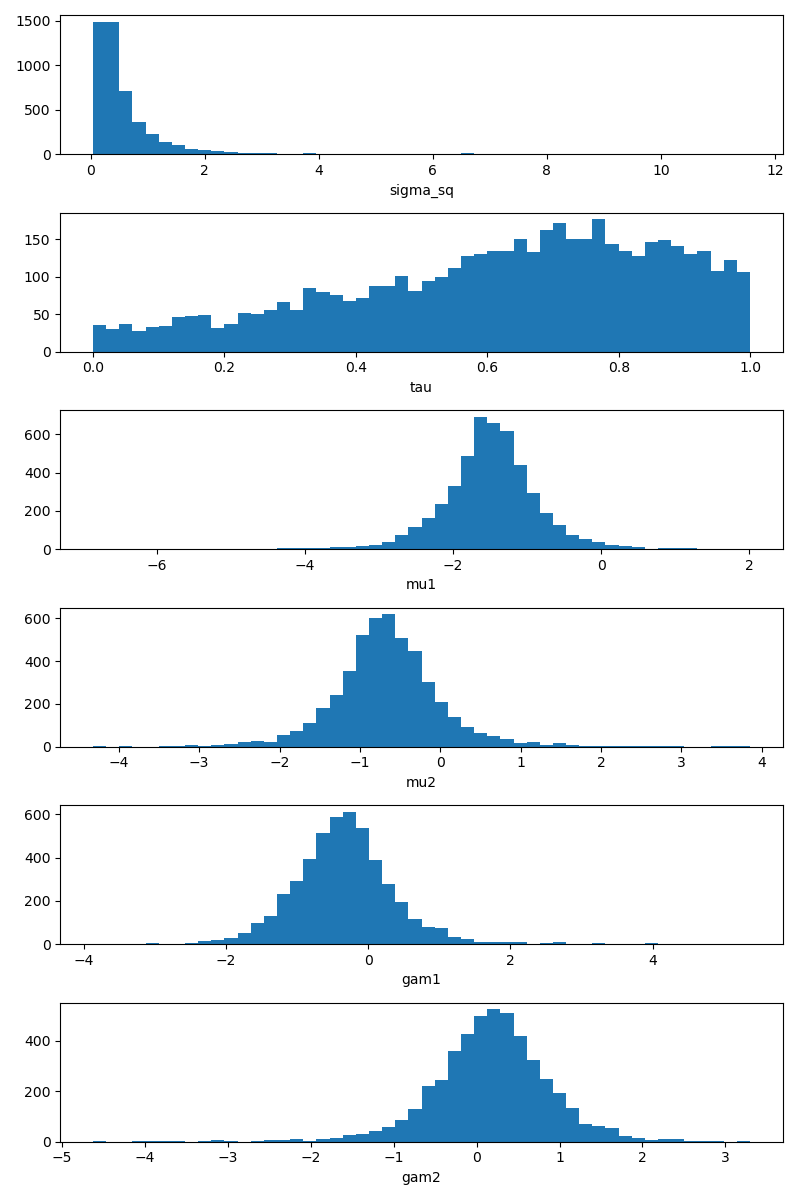
\includegraphics[scale=0.7]{hmc_sampled_histogram.png}
    \caption{Histogram of Hamiltonian Monte Carlo posterior samples}
\end{figure}

The traceplots in figure 4 give an indication of how well the sampler 
explored the posterior density. I am comforted by the fact that 
there are no long periods of repeated values (getting stuck) 
despite us not implementing no-turn logic. 
\begin{figure}[H]
    \centering
    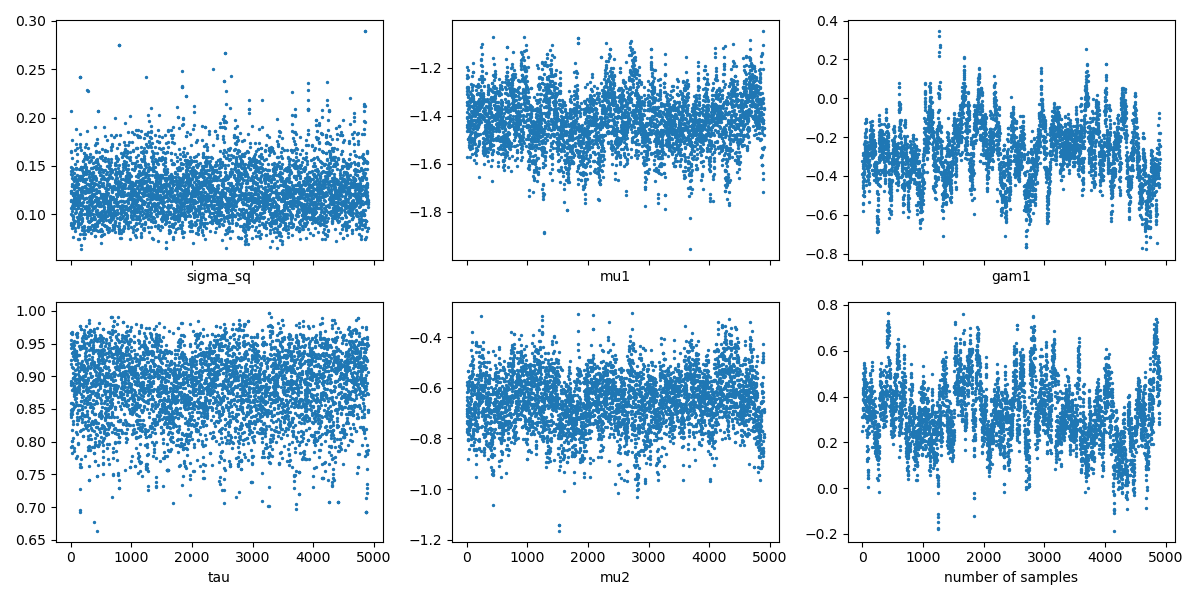
\includegraphics[scale=0.7]{hmc_sampled_traceplot.png}
    \caption{Traceplot for Hamiltonian Monte Carlo sampling}
\end{figure}

\textbf{Final remarks}. HMC was much slower to run than Metropolis-
Hastings due to the gradient evaluation at each iteration (4,205 sec 
for 5000 samples), however, our acceptance ratio was much higher 
(approx. 0.95 vs 0.45). Moreover, our samples were far less likely 
to be autocorrelated (approx. 46 vs 5 effective samples per 100 
iterations). This is because we are taking directed rather than 
random steps through the posterior.



\section{Gibbs Sampling}
To implement the Gibbs Sampling we need to derive the conditional 
distributions for each parameter from which to sample. 

\textbf{Conditional distributions} Idea: start with joint posterior 
density, then remove constants (e.g. terms with only fixed parameters) 
and rearrange to derive density conditional distribution we can sample 
from. To simplify notation, let $\theta[-x]$ represent all parameters 
of $\theta$ exluding parameter $x$ and let $y_i'$ represent centered data 
(e.g. $y_1' = y_1 - \mu$). \newline

Derive conditional distribution for $\sigma^2$.
\begin{align*}
    p(\sigma^2|y,\theta[-\sigma^2]) & \propto \prod_{t_i=1} N(\mu, \sigma^2 \mathbb{I}) \cdot \prod_{t_i=2} N(\gamma, \sigma^2 \mathbb{I}) \cdot \prod_{t_i=3} N(0.5\mu + 0.5\gamma, \sigma^2 \mathbb{I}) \cdot \prod_{t_i=4} N(\tau\mu + (1-\tau)\gamma, \sigma^2 \mathbb{I}) \cdot p(\sigma^2) \\
        & \propto |\sigma^2 \mathbb{I}_2|^{-n/2} \cdot \frac{1}{\sigma^2} \cdot \exp\left(-\frac{1}{2\sigma^2}\sum_{i=1}^n y_i'^T \mathbb{I}^{-1} y_i'\right) \\
        & \propto (\frac{1}{\sigma^2})^{n+1} \cdot \exp\left(-\frac{1}{\sigma^2} \cdot \frac{1}{2} \sum_{i=1}^n \|y_i'\|^2_2\right) \\
        & = x^{\alpha + 1} \cdot \exp(-x \beta) \\
    \therefore \sigma^2 | y, \theta[-\sigma^2] & \sim \text{InvGamma}\left(n, \quad \frac{1}{2} \sum_{i=1}^n \|y_i'\|^2_2\right)
\end{align*}

Derive conditional distribution for $\tau$.
\begin{align*}
    p(\tau|y,\theta[-\tau]) & \propto \exp\left(-\frac{1}{2\sigma^2} \sum_{t_i=4} (y_i - (\tau\mu + (1-\tau)\gamma))^T \mathbb{I}^{-1} (y_i - (\tau\mu + (1-\tau)\gamma)) \right)\\
        & \propto \exp\left(-\frac{1}{2} \cdot \frac{\|\gamma - \mu\|^2_2}{\sigma^2} \sum_{t_i=4} (\tau \vec{i} - \alpha_i)^T \mathbb{I}^{-1} (\tau \vec{i} - \alpha_i) \right) && \text{let $\vec{i} = (1, 1)$} \\
        & \propto \exp\left(-\frac{1}{2} \cdot \frac{\|\gamma - \mu\|^2_2}{\sigma^2} \sum_{t_i=4} \left( \|\tau \vec{i}\|^2_2 - 2\tau \vec{i}^T \alpha_i + \|\alpha_i\|^2_2\right) \right) && \text{$\|\alpha_i\|^2_2$ constant} \\
        & \propto \exp\left(-\frac{1}{2} \cdot \frac{\|\gamma - \mu\|^2_2}{\sigma^2} \left( n_4 \tau^2 - 2\tau \vec{i}^T \sum_{t_i=4} \alpha_i \right) \right) && \\
        & \propto \exp\left(-\frac{1}{2} \cdot \frac{n_4 \|\gamma - \mu\|^2_2}{\sigma^2} \left(\tau - \frac{\sum_{t_i=4} \alpha_i}{n_4} \right)^2 \right) && \text{complete the square}
\end{align*}
$$\therefore \tau | y, \theta[-\tau] \sim \text{TruncNormal}\left(\frac{\sum_{t_i=4} \alpha_i}{n_4}, \frac{\sigma^2}{n_4 \|\gamma - \mu\|^2_2}, 0, 1\right) \quad \text{where } \alpha_i = y_i^T \mu - \gamma^T\gamma - y_i^T\gamma - \mu^T\gamma$$

Derive conditional distribution for $\mu$.
\begin{align*}
    p(\mu|y,\theta[-\mu]) & \propto \exp\left(-\frac{1}{2\sigma^2} \sum_{t_i \in \{1,3,4\}} (y_i - \bar{y}_i)^T \mathbb{I}^{-1} (y_i - \bar{y}_i) \right) && \text{$\bar{y}_i$ = group mean}\\
        & \propto \exp\left(-\frac{1}{2} \cdot \frac{1}{\sigma^2} \sum_{t_i \in \{1,3,4\}} (\mu - \bar{\mu}_i^{t_i})^T \mathbb{I}^{-1} (\mu - \bar{\mu}_i^{t_i}) \right) && \text{rearrange for $\mu$}\\
        & \propto \exp\left(-\frac{1}{2} \cdot \frac{1}{\sigma^2} \sum_{t_i \in \{1,3,4\}} \left(\|\mu\|^2_2 - 2\mu^T \bar{\mu}_i^{t_i} + \|\bar{\mu}_i^{t_i}\|^2_2 \right)\right) && \text{$\|\bar{\mu}_i^{t_i}\|^2_2$ constant}\\
        & \propto \exp\left(-\frac{1}{2} \cdot \frac{1}{\sigma^2} \left((n_1 + 0.5^2 n_3 + \tau^2 n_4)\|\mu\|^2_2 - 2\mu^T \sum_{t_i \in \{1,3,4\}} \bar{\mu}_i^{t_i} \right)\right) && \text{take $\|\mu\|^2_2$ outside sum}\\
        & \propto \exp\biggl(-\frac{1}{2} \cdot \frac{n_1 + 0.5^2 n_3 + \tau^2 n_4}{\sigma^2} && \text{complete the square} \\
        & \quad \left(\mu - \frac{\sum_{t_i \in \{1,3,4\}} \bar{\mu}_i^{t_i}}{n_1 + 0.5^2 n_3 + \tau^2 n_4} \right)^T \mathbb{I}^{-1} \left(\mu - \frac{\sum_{t_i \in \{1,3,4\}} \bar{\mu}_i^{t_i}}{n_1 + 0.5^2 n_3 + tau^2 n_4} \right)\biggr) && \\
    \therefore \mu | y, \theta[-\mu] & \sim \text{Normal}\left( \frac{\sum_{t_i \in \{1,3,4\}} \bar{\mu}_i^{t_i}}{n_1 + 0.5^2 n_3 + \tau^2 n_4}, \quad \frac{\sigma^2}{n_1 + 0.5^2 n_3 + \tau^2 n_4} \right) \\
    \text{where} & \quad \bar{\mu}_i^{t=1} = y_i \text{;} \quad \bar{\mu}_i^{t=3} = (y_i - 0.5\gamma) / 0.5 \text{;} \quad \bar{\mu}_i^{t=4} = (y_i - (1-\tau)\gamma) / \tau 
\end{align*}

Derive conditional distribution for $\gamma$.
\begin{align*}
    p(\gamma|y,\theta[-\gamma]) & \propto \exp\left(-\frac{1}{2\sigma^2} \sum_{t_i \in \{2,3,4\}} (y_i - \bar{y}_i)^T \mathbb{I}^{-1} (y_i - \bar{y}_i) \right) \\ %&& \text{$\bar{y}_i$ = group mean}\\
        & \propto \exp\left(-\frac{1}{2} \cdot \frac{1}{\sigma^2} \sum_{t_i \in \{2,3,4\}} (\gamma - \bar{\gamma}_i^{t_i})^T \mathbb{I}^{-1} (\gamma - \bar{\gamma}_i^{t_i}) \right) \\ %&& \text{rearrange for $\gamma$}\\
        & \propto \exp\left(-\frac{1}{2} \cdot \frac{1}{\sigma^2} \sum_{t_i \in \{2,3,4\}} \left(\|\gamma\|^2_2 - 2\gamma^T \bar{\gamma}_i^{t_i} + \|\bar{\gamma}_i^{t_i}\|^2_2 \right)\right) \\ %&& \text{$\|\bar{\gamma}_i^{t_i}\|^2_2$ constant}\\
        & \propto \exp\left(-\frac{1}{2} \cdot \frac{1}{\sigma^2} \left((n_2 + 0.5^2 n_3 + (1-\tau)^2 n_4)\|\gamma\|^2_2 - 2\gamma^T \sum_{t_i \in \{2,3,4\}} \bar{\gamma}_i^{t_i} \right)\right) \\ %&& \text{take $\|\gamma\|^2_2$ outside sum}\\
        & \propto \exp\biggl(-\frac{1}{2} \cdot \frac{n_2 + 0.5^2 n_3 + (1-\tau)^2 n_4}{\sigma^2} \\ %&& \text{complete the square} \\
        & \quad \left(\gamma - \frac{\sum_{t_i \in \{2,3,4\}} \bar{\gamma}_i^{t_i}}{n_2 + 0.5^2 n_3 + (1-\tau)^2 n_4} \right)^T \mathbb{I}^{-1} \left(\gamma - \frac{\sum_{t_i \in \{2,3,4\}} \bar{\gamma}_i^{t_i}}{n_2 + 0.5^2 n_3 + (1-\tau)^2 n_4} \right)\biggr) && \\
    \therefore \gamma | y, \theta[-\gamma] & \sim \text{Normal}\left( \frac{\sum_{t_i \in \{2,3,4\}} \bar{\gamma}_i^{t_i}}{n_2 + 0.5^2 n_3 + (1-\tau)^2 n_4}, \quad \frac{\sigma^2}{n_2 + 0.5^2 n_3 + (1-\tau)^2 n_4} \right) \\
    \text{where} & \quad \bar{\gamma}_i^{t=2} = y_i \text{;} \quad \bar{\gamma}_i^{t=3} = (y_i - 0.5\mu) / 0.5 \text{;} \quad \bar{\gamma}_i^{t=4} = (y_i - \tau\mu) / (1-\tau) 
\end{align*}

Having derived our conditional distributions, the gibbs implementation
itself is very straightforward. We iterate through and update one or 
multiple parameters at a time (see below).  
\begin{python}
def gibbs_sampling(data, n_samples, initial_position):
    samples = [initial_position]

    it = 0
    while it < n_samples:
        it += 1
        curr_theta = samples[-1].copy()
        idx = (it-1) % 4  # systematic

        if idx == 0:
            sigma_sq_proposal = sample_ssq_conditional_posterior(data, curr_theta)
            curr_theta[0] = sigma_sq_proposal

        elif idx == 1:
            tau_proposal = sample_tau_conditional_posterior(data, curr_theta)
            curr_theta[1] = tau_proposal

        elif idx == 2:
            mu_proposal = sample_mu_conditional_posterior(data, curr_theta)
            curr_theta[2:4] = mu_proposal

        elif idx == 3:
            gam_proposal = sample_gam_conditional_posterior(data, curr_theta)
            curr_theta[4:6] = gam_proposal

        else:
            print("Error: trying to update out-of-bounds parameter!")
        samples.append(curr_theta)

    return np.array(samples)
\end{python}

The Gibbs Sampling algorithm has a number of design 
choices, including (a) systematic vs random scan, and
(b) block vs individual parameter updates. Note: there 
is no hyperparameter tuning for step size here because 
we take a completely new sample (from an adaptive proposal 
distribution) at each step.

\begin{enumerate}[label=(\alph*)]
\item \textbf{Systematic vs random scan}: While random scan ensures 
detail balance of our markov chain, I preferred to use a 
systematic scan since it was more efficient, especially over 
smaller sampling experiments (guarantees an equal number of 
updates for each).

\item \textbf{Block updates for mu and gamma}: Since $\mu_1, \mu_2$ 
and $\gamma_1, \gamma_2$ would always come from the same 
distribution I found it more efficient to update these together, 
drawing from a 2-dim multivariate normal rather than separately. 
This does mean that our proposals
\end{enumerate}

\textbf{Results}: Using the above design choices, we produce the following 
samples from our posterior (figure 5).
\begin{figure}[H]
    \centering
    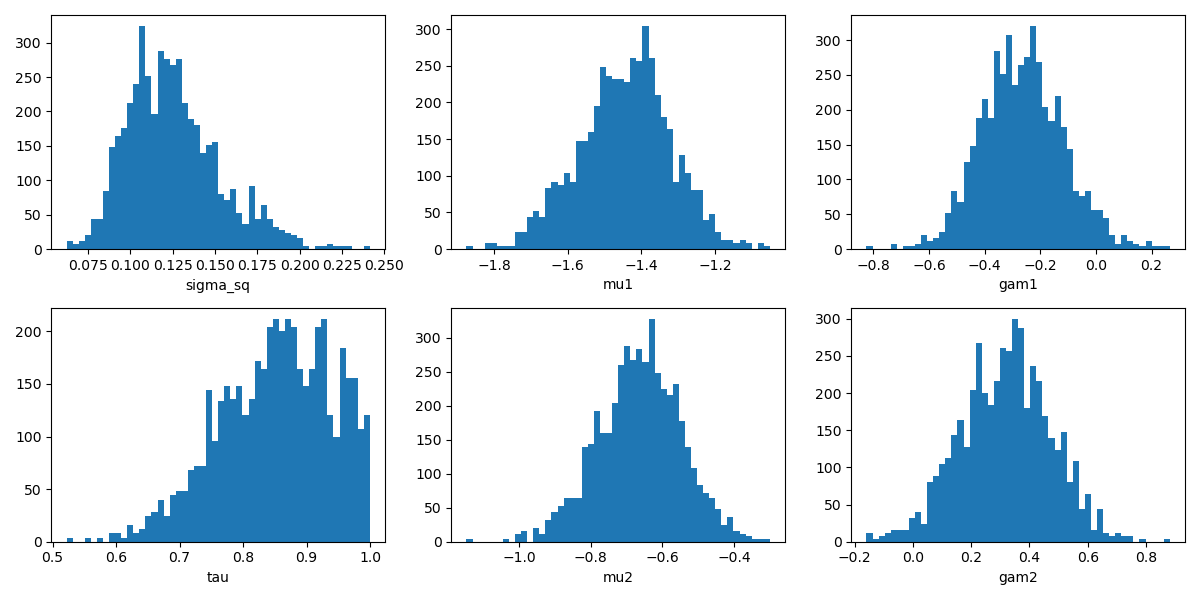
\includegraphics[scale=0.7]{gibbs_sampled_histogram.png}
    \caption{Histogram of Hamiltonian Monte Carlo posterior samples}
\end{figure}

The traceplots in figure 6 give an indication of how well the sampler 
explored the posterior density. I am comforted by the fact that 
there are no long periods of repeated values (getting stuck) 
despite us not implementing no-turn logic. 
\begin{figure}[H]
    \centering
    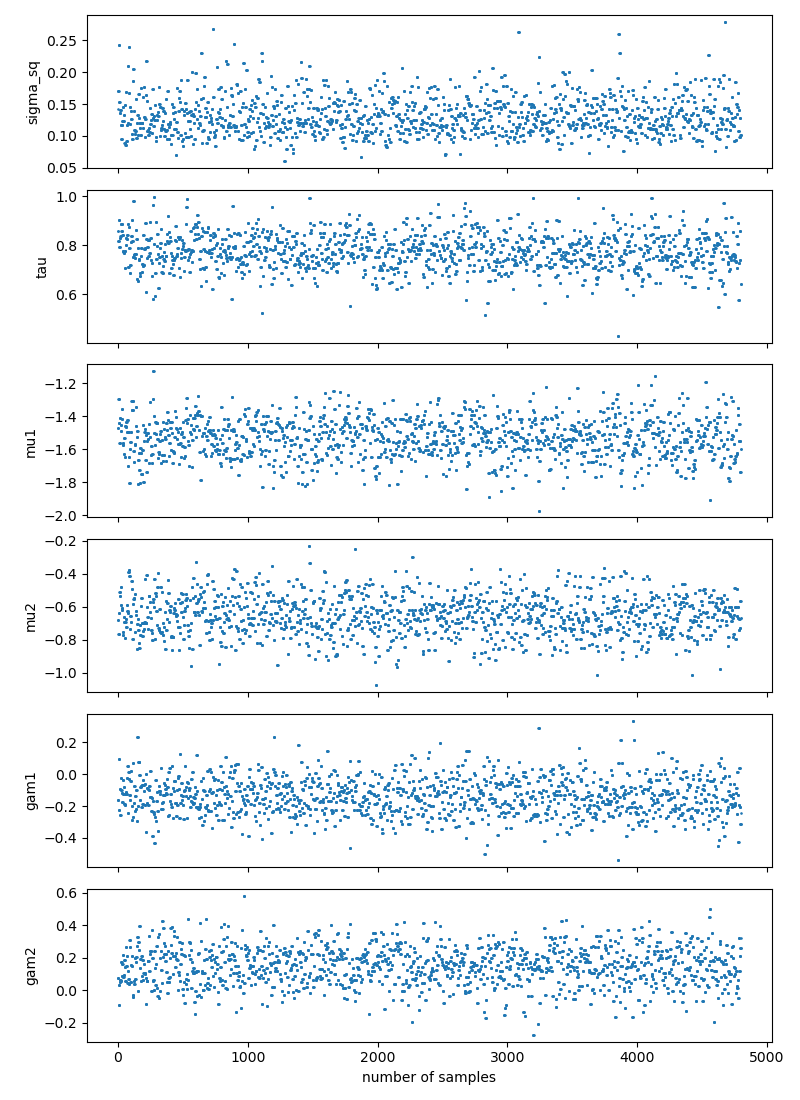
\includegraphics[scale=0.7]{gibbs_sampled_traceplot.png}
    \caption{Traceplot for Hamiltonian Monte Carlo sampling}
\end{figure}

\textbf{Final remarks}. The Gibbs sampling algorithm is lightning 
fast compared to MH and HMC (25.0 sec!). This is because it does 
not execute an acceptance criterion! The main tradeoff is that our 
samples have significant autocorrelation (approx. 16 effective 
samples per 100 iterations). Note, the number of effective samples 
still surpasses MH but is almost 1/3 of our HMC result.



\section{Importance Sampling}

Importance Sampling is typically used to estimate summary statistics. 
For example, if $I_A(x)$ is the indicator function of x lying in 
some region A, and we know the target density $p(x)$, we can pick a 
proposal distribution $Q$ to sample from and weight our samples 
in the following way.
$$ E[I_A(x)] = \int I_A(x) p(x) dx = \int I_A(x) \frac{p(x)}{q(x)} q(x) dx \approx \frac{1}{n} \sum I_A(x) \frac{p(x)}{q(x)} $$ 

Adapting this theory to our problem, we want to derive our target 
density $p(\theta|y)$ (likliehood x prior) and find a suitable 
proposal distribution Q that we can sample from to produce a set 
of samples and corresponding weights for each. Scaling each sample 
by its respective weight will give us posterior samples! \newline

\begin{python}
    def multistep_importance_sampling(data, n_samples, initial_position):
    samples, weights = [initial_position], [0]
    for it in range(n_samples):

        # sample from proposal dist q
        theta = sample_from_proposal_dist(data)
        samples.append(theta)

        # evaluate p(theta) and q(theta) to compute weight
        p_theta = joint_posterior_density(data, theta)  # trial density
        q_theta = compute_proposal_density(data, theta)  # proposal
        weights.append(p_theta/q_theta)

    return np.array(samples), np.array(weights)
\end{python}

The importance sampling method requires us to make a number of design 
choices, including (a) selecting a proposal distribution, (b) whether to 
use a normalized scheme, and (c) choice of prior for $\tau$.

\begin{enumerate}[label=(\alph*)]
    \item \textbf{Proposal distribution}. Want to find a proposal distribution that is as similar 
    as possible (but with greater variance) to distribution described by our target density. 
    Idea: split evaluation of the posterior into two separate steps: 
    \begin{itemize}
        \item \textbf{Step 1}: Use only groups 1 and 2 to generate a closed form partial posterior ($\mu, \gamma, \sigma^2$ only). Combine with some $p(\tau)$ to generate our proposal distribution Q
        \item \textbf{Step 2}: Use output from step 1 as our new prior, then update using likelihood of data from groups 3 and 4 given parameters $\theta$ to generate our target density (equivalent to joint posterior) 
    \end{itemize}

    This two-step approach is attractive because it uses our data effectively to inform 
    our proposal distribution. Let $\theta = (\mu, \gamma, \tau, \sigma^2)$.
    \begin{align*}
        p(\theta|Y_{1,2,3,4}) & \propto p(\mu, \gamma, \sigma^2|Y_{1,2}) \cdot p(\tau) \cdot L(Y_{3,4}|\theta) \\
            & \propto p(\mu, \gamma, \sigma^2|Y_{1,2}) \cdot p(\tau) \cdot \prod_{t\in{3,4}} p(y_i|\theta) \\
            & \propto q(\theta) \cdot \prod_{t_i\in{3,4}} p(y_i|\theta) && \text{choose proposal $q(\theta)$}
    \end{align*}

    Want to find closed form distribution for $p(\mu, \gamma, \sigma^2|Y_{1,2})$. 
    First recognize we can separate $\sigma^2$ from $\mu$ and $\gamma$.
    $$ p(\mu, \gamma, \sigma^2|Y_{1,2}) = p(\mu, \gamma|Y_{1,2}) \cdot p(\sigma^2|\mu, \gamma, Y_{1,2}) $$
    
    Derive $p(\sigma^2|\mu, \gamma, Y_{1,2})$: $\sigma^2$ conditional on $\mu$, $\gamma$ and groups 1, 2.
    \begin{align*}
        p(\sigma^2|\mu, \gamma, Y_{1,2}) & \propto \frac{1}{\sigma^2} \cdot \left(\frac{1}{\sigma^2}\right)^{n_1 + n_2} \exp\left(-\frac{1}{2\sigma^2}(\sum_{t_i=1} \|y_i-\mu\|^2_2 + \sum_{t_i=2} \|y_i-\gamma\|^2_2)\right) \\
            & \text{let $M_{\sigma^2}=\sum_{t_i=1} \|y_i-\mu\|^2_2 + \sum_{t_i=2} \|y_i-\gamma\|^2_2$} \\
            & \propto \left(\frac{1}{\sigma^2}\right)^{n_1 + n_2 + 1} \exp\left(-\frac{M_{\sigma^2}}{2} \cdot \frac{1}{\sigma^2}\right) \\
            & \propto \text{InvGamma}\left(n_1+n_2, \quad \frac{M_{\sigma^2}}{2} \right)
    \end{align*}

    Derive $p(\mu, \gamma|Y_{1,2})$: the marginal distribution of $\mu$ and $\gamma$.
    \begin{align*}
        p(\mu, \gamma|Y_{1,2}) & = \int_0^{\infty} p(\mu, \gamma, \sigma^2|Y_{1,2}) d\sigma^2 \\
            & \propto \int_0^{\infty} \left(\frac{1}{\sigma^2}\right)^{n_1+n_2+1} \exp\left(-\frac{1}{2\sigma^2}(\sum_{t_i=1} \|y_i-\mu\|^2_2 + \sum_{t_i=2} \|y_i-\gamma\|^2_2)\right) d\sigma^2 \\
        \textrm{ recall  }\quad& \frac{\Gamma(\alpha)}{\beta^\alpha} = \int_0^\infty (\sigma^2)^{-\alpha - 1} \exp\left(\frac{\beta}{\sigma^2}\right)d\sigma^2\\
            & \propto \; \Gamma(n_1 + n_2) \left(-\frac{1}{2}  \sum_{t_i=1} \lVert y_i - \mu\rVert^2 + \sum_{t_i=2}\lVert y_i - \gamma \rVert^2\right)^{-(n_1 + n_2)} \\
            & \propto \; (\sum_{t_i=1}\lVert y_i - \overline{Y_1} \rVert^2 + \sum_{t_i=2}\lVert y_i - \overline{Y_2} \rVert^2 + n_1\lVert \overline{Y_1} - \mu \rVert^2 + n_2\lVert \overline{Y_2} - \gamma \rVert^2)^{-(n_1 + n_2)}\\
        \textrm{ define  }\quad& M_{\mu, \gamma} = \sum_{t_i=1}\lVert y_i - \overline{Y_1} \rVert^2 + \sum_{t_i=2}\lVert y_i - \overline{Y_2} \rVert^2\\
            & \propto \; (M_{\mu, \gamma} + n_1\lVert \overline{Y_1} - \mu \rVert^2 + n_2\lVert \overline{Y_2} - \gamma \rVert^2)^{-(n_1 + n_2)}\\
            & \propto \; \left(M_{\mu, \gamma} + \left[\left(\begin{matrix}\mu\\ \gamma\end{matrix}\right) - \left(\begin{matrix*}\overline{Y_1}\\ \overline{Y_2}\end{matrix*}\right)\right]^T \left(\begin{matrix*} n_1 & 0 & 0 & 0 \\ 0 & n_1 & 0 & 0 \\ 0 & 0 & n_2 & 0 \\ 0 & 0 & 0 & n_2 \end{matrix*}\right) \left[\left(\begin{matrix}\mu\\ \gamma\end{matrix}\right) - \left(\begin{matrix*}\overline{Y_1}\\ \overline{Y_2}\end{matrix*}\right)\right]\right)^{-(n_1 + n_2)}\\
            & \propto \; \biggl(1 + \frac{2(n_1 + n_2) - 4}{M_{\mu, \gamma}(2(n_1 + n_2) - 4)}\left[\left(\begin{matrix}\mu\\ \gamma\end{matrix}\right) - \left(\begin{matrix*}\overline{Y_1}\\ \overline{Y_2}\end{matrix*}\right)\right]^T \left(\begin{matrix*} n_1{-1} & 0 & 0 & 0 \\ 0 & n_1^{-1} & 0 & 0 \\ 0 & 0 & n_2{-1} & 0 \\ 0 & 0 & 0 & n_2{-1} \end{matrix*}\right)^{-1} \\
            & \quad \quad \quad \left[\left(\begin{matrix}\mu\\ \gamma\end{matrix}\right) - \left(\begin{matrix*}\overline{Y_1}\\ \overline{Y_2}\end{matrix*}\right)\right]\biggr)^{-(n_1 + n_2)}\\
            & \propto \; \left[1 + \frac{1}{\nu}(x - \eta)^T\Sigma^{-1}(x - \eta)\right]^{-\frac{\nu + 4}{2}} \quad \text{recognize t-distribution density}\\
        \text{ where }\quad& \nu=2(n_1 + n_2) + 4, \Sigma=\frac{M_{\mu, \gamma}}{2(n_1 + n_2) - 4}\left(\begin{matrix*} n_1{-1} & 0 & 0 & 0 \\ 0 & n_1^{-1} & 0 & 0 \\ 0 & 0 & n_2{-1} & 0 \\ 0 & 0 & 0 & n_2{-1} \end{matrix*}\right), \eta=\left(\begin{matrix*}\overline{Y_1}\\ \overline{Y_2}\end{matrix*}\right)\\
        \therefore p(\mu, \gamma \mid Y_{1,2}) &\sim t_4\left(\left(\begin{matrix*}
            \overline{Y_1}\\ \overline{Y_2} \end{matrix*}\right), \frac{M_{\mu, \gamma}}{2(n_1 + n_2) - 4}\left(\begin{matrix*}
            n_1^{-1} & 0 & 0 & 0 \\ 0 & n_1^{-1} & 0 & 0 \\ 0 & 0 & n_2^{-1} & 0 \\ 0 & 0 & 0 & n_2^{-1}
            \end{matrix*}\right)\right)
    \end{align*}

    Putting these parts together we have the following proposal distribution,
    $$ q(\theta) \sim t_4\left(\left(\begin{matrix*}
        \overline{Y_1}\\ \overline{Y_2} \end{matrix*}\right), \frac{M_{\mu, \gamma}}{2(n_1 + n_2) - 4}\left(\begin{matrix*}
        n_1^{-1} & 0 & 0 & 0 \\ 0 & n_1^{-1} & 0 & 0 \\ 0 & 0 & n_2^{-1} & 0 \\ 0 & 0 & 0 & n_2^{-1}
        \end{matrix*}\right)\right) \cdot \text{InvGamma}\left(n_1+n_2, \quad \frac{M_{\sigma^2}}{2} \right) $$

    \item \textbf{Normalized importance sampling}. xx cannot solve for closed form after groups 1 and 2.
    Idea: let our target $p(x) = f(x) / z_p$ and $q(x) = g(x) / z_q$ where 
    we can evaluate $f(x), g(x)$ but not $p(x), q(x)$ are $z_p, z_q$ are 
    constants. \newline

    If we draw $x_i$ $i=1,2,...n$ iid samples from Q distribution, then compute 
    weights $u_i = f(x_i) / g(x_i)$ and apply these to our samples, we can 
    recover the weights as if we had been able to evaluate $p(x)$ and 
    directly compute $w_i = p(x_i) / q(x_i)$:
    $$ \hat{x_i} = \frac{x_i \cdot w_i}{\sum_{i=1}^n w_i} = \frac{\frac{z_p}{z_q} \cdot x_i \cdot \frac{f(x_i)}{g(x_i)}}{\sum_{i=1}^n \frac{f(x_i)}{g(x_i)}} = \frac{x_i \cdot u_i}{\sum_{i=1}^n u_i}$$

    This is important for our particular problem since it is not possible 
    to compute the closed form posterior (target density) adn so instead 
    we need to make do with some $f(x) \propto p(x)$, which we take to be
    the likelihood x prior.

    \item \textbf{Choice of tau prior}. While we were able to solve for a 
    closed form of the posterior for groups 1 and 2, this does not give us 
    any additional information about $\tau$ to use as a prior for Step 2. 
    I tried both using a beta centered at zero $\text{Beta}(5, 2)$ and a 
    beta centered at 0.8 $\text{Beta}(5, 2)$ where we know $\tau$ should 
    be from our other sampling experiments.  
\end{enumerate}


\section{Comparison of methodologies} Autocorrelation, speed to evaluate, sample efficiency,
 biased estimator, ...table!
 



\end{document}
